%%- Premier chapitre de démonstration -%%
\chapter{Test de long titre de Chapitre, avec retour à la ligne. Lorem ipsum dolor sit amet, consectetur adipiscing elit. Pellentesque justo justo, porta sagittis feugiat eget, ornare rhoncus ligula. Nunc non odio sed lacus rutrum rhoncus.}


\section{Tests de mise en page}

Dans cette section, différents environnements de mise en page sont présentés.

\subsection{Figure simple}

    Insertion d'une figure dont le numéro est Fig. \ref{figureSimple}
    \begin{figure}
    	\centering % Les figures doivent être centrées
    	
\includegraphics[width=0.5\textwidth]{figures/logoUNA.jpg}
            \caption{Insertion d'une figure simple}\label{figureSimple}
    \end{figure}

\lipsum[1]
\subsection{Figures avec légende longue}
    Exemple de déclaration de figure
    \begin{figure}
        \centering % Les figures doivent être centrées
        
\includegraphics[width=0.5\textwidth]{figures/logoESPA.png} % 
        \\ \parbox{0.75\textwidth}{\caption{Test de longue légende, avec utilisation de framebox et parbox pour restreindre la largeur de la légende.}\label{logoESPA}} % Utilisation d'une parbox pour restreindre la largeur de la légende.
    \end{figure}
\lipsum[2]
\subsection{Insertion de plusieurs figures}

Ci-après est un exemple d'insertion de deux figures cote à cote.

        \begin{figure*}[!h]
		\begin{center}
			\subfloat[Recherche de la meilleure réponse]{
				\label{org-brm001}
					\hspace{0.5cm}
					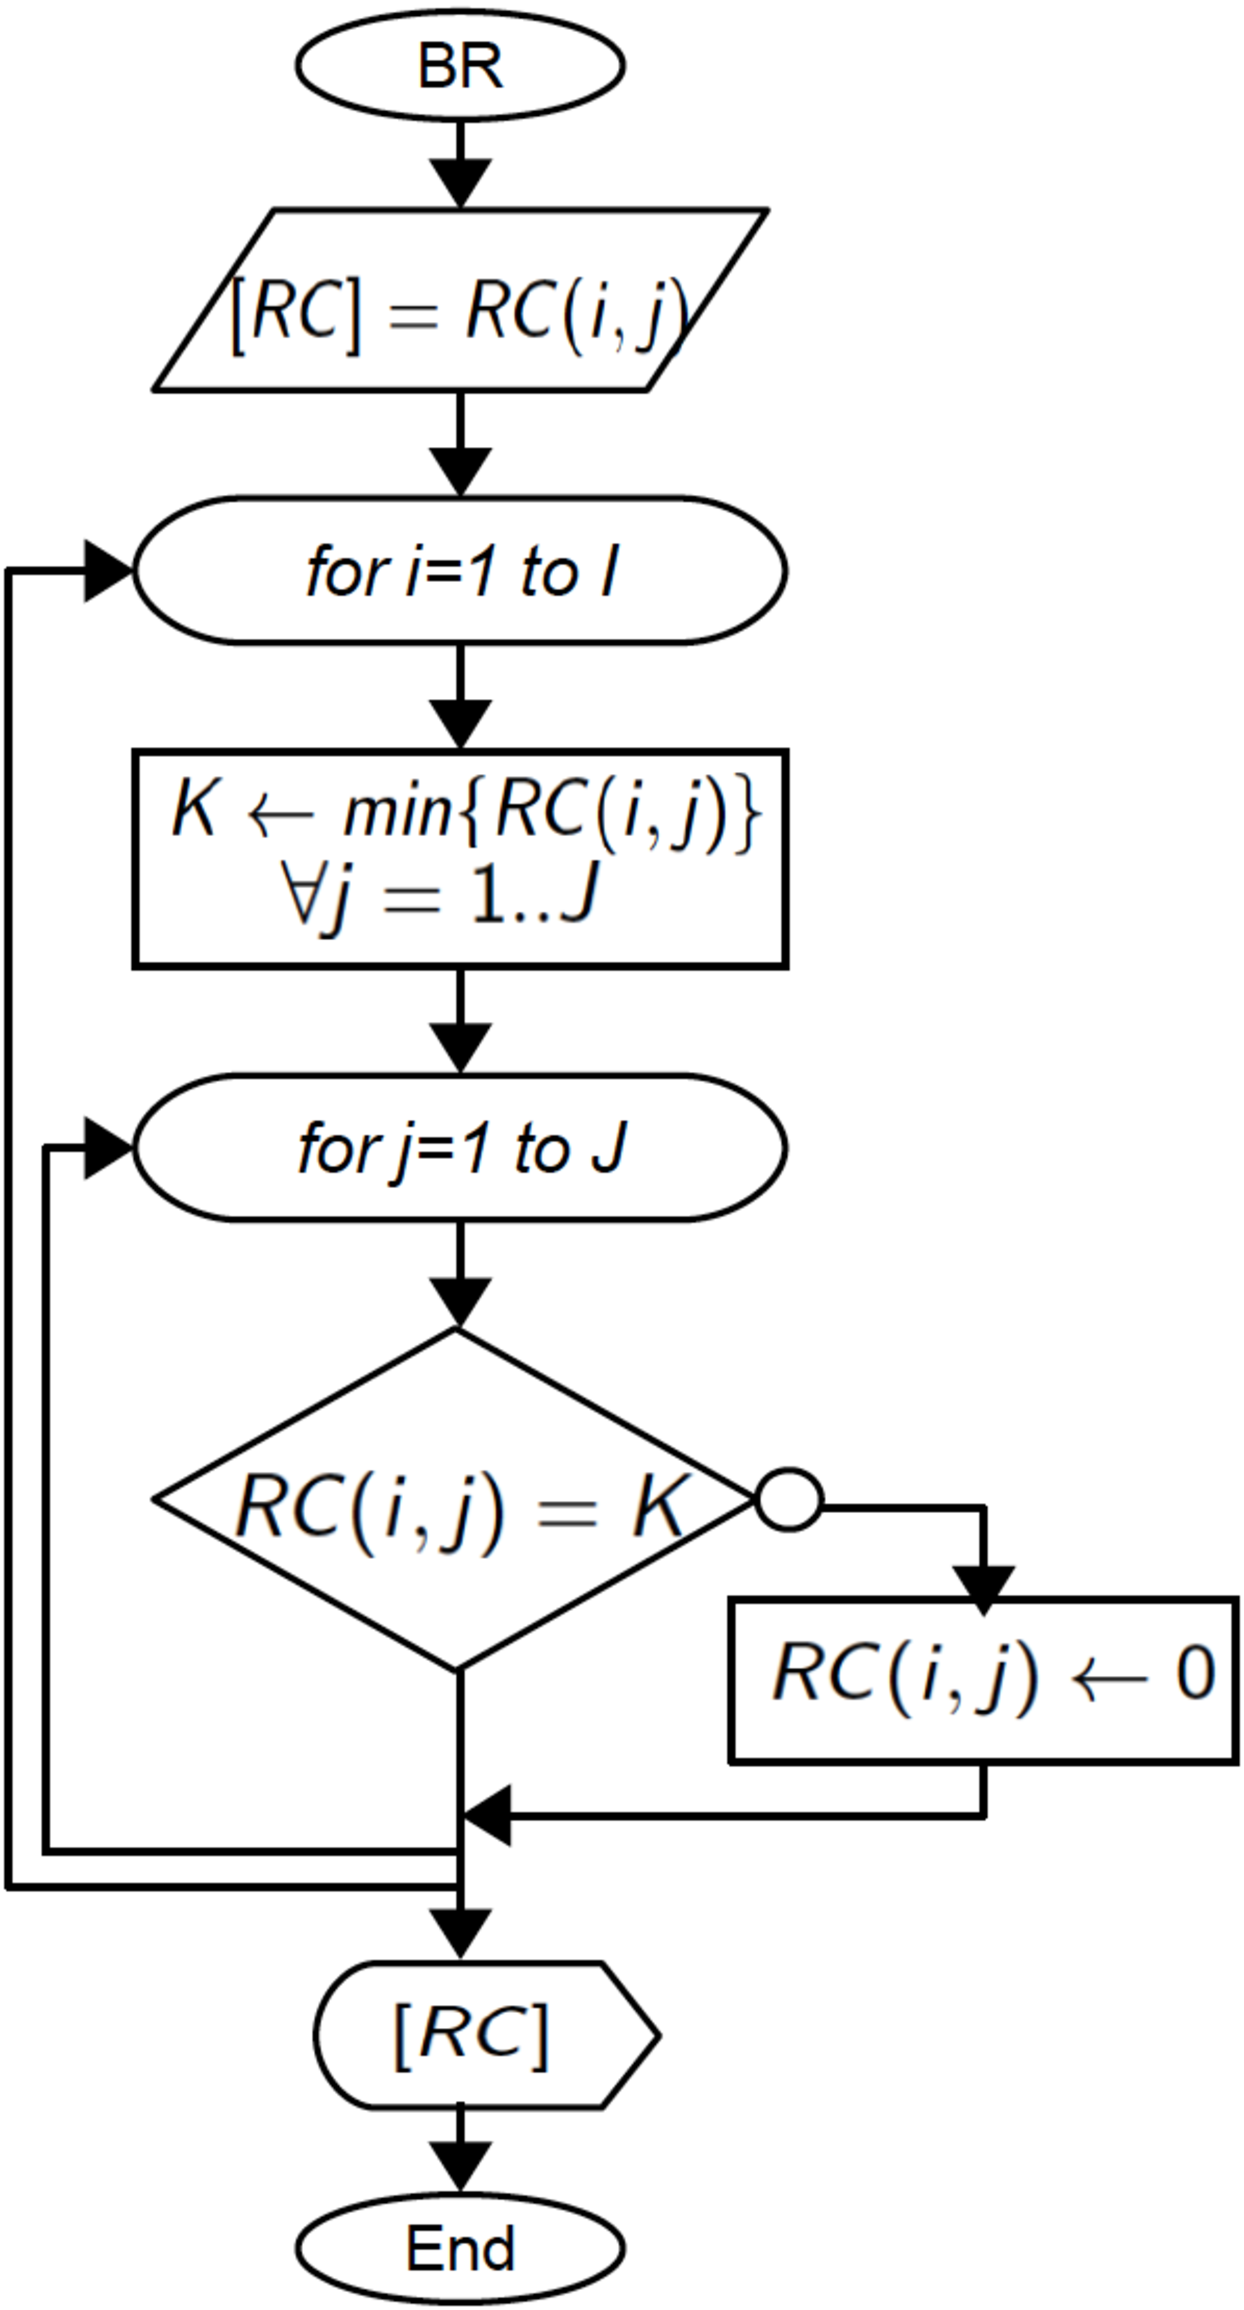
\includegraphics[width=0.41\textwidth]{figures/org-brm001}
					\hspace{0.4cm}
			}\hfill
			\subfloat[Sélection des meilleures réponses]{
				\label{org-brm002}
					\hspace{0.7cm}
					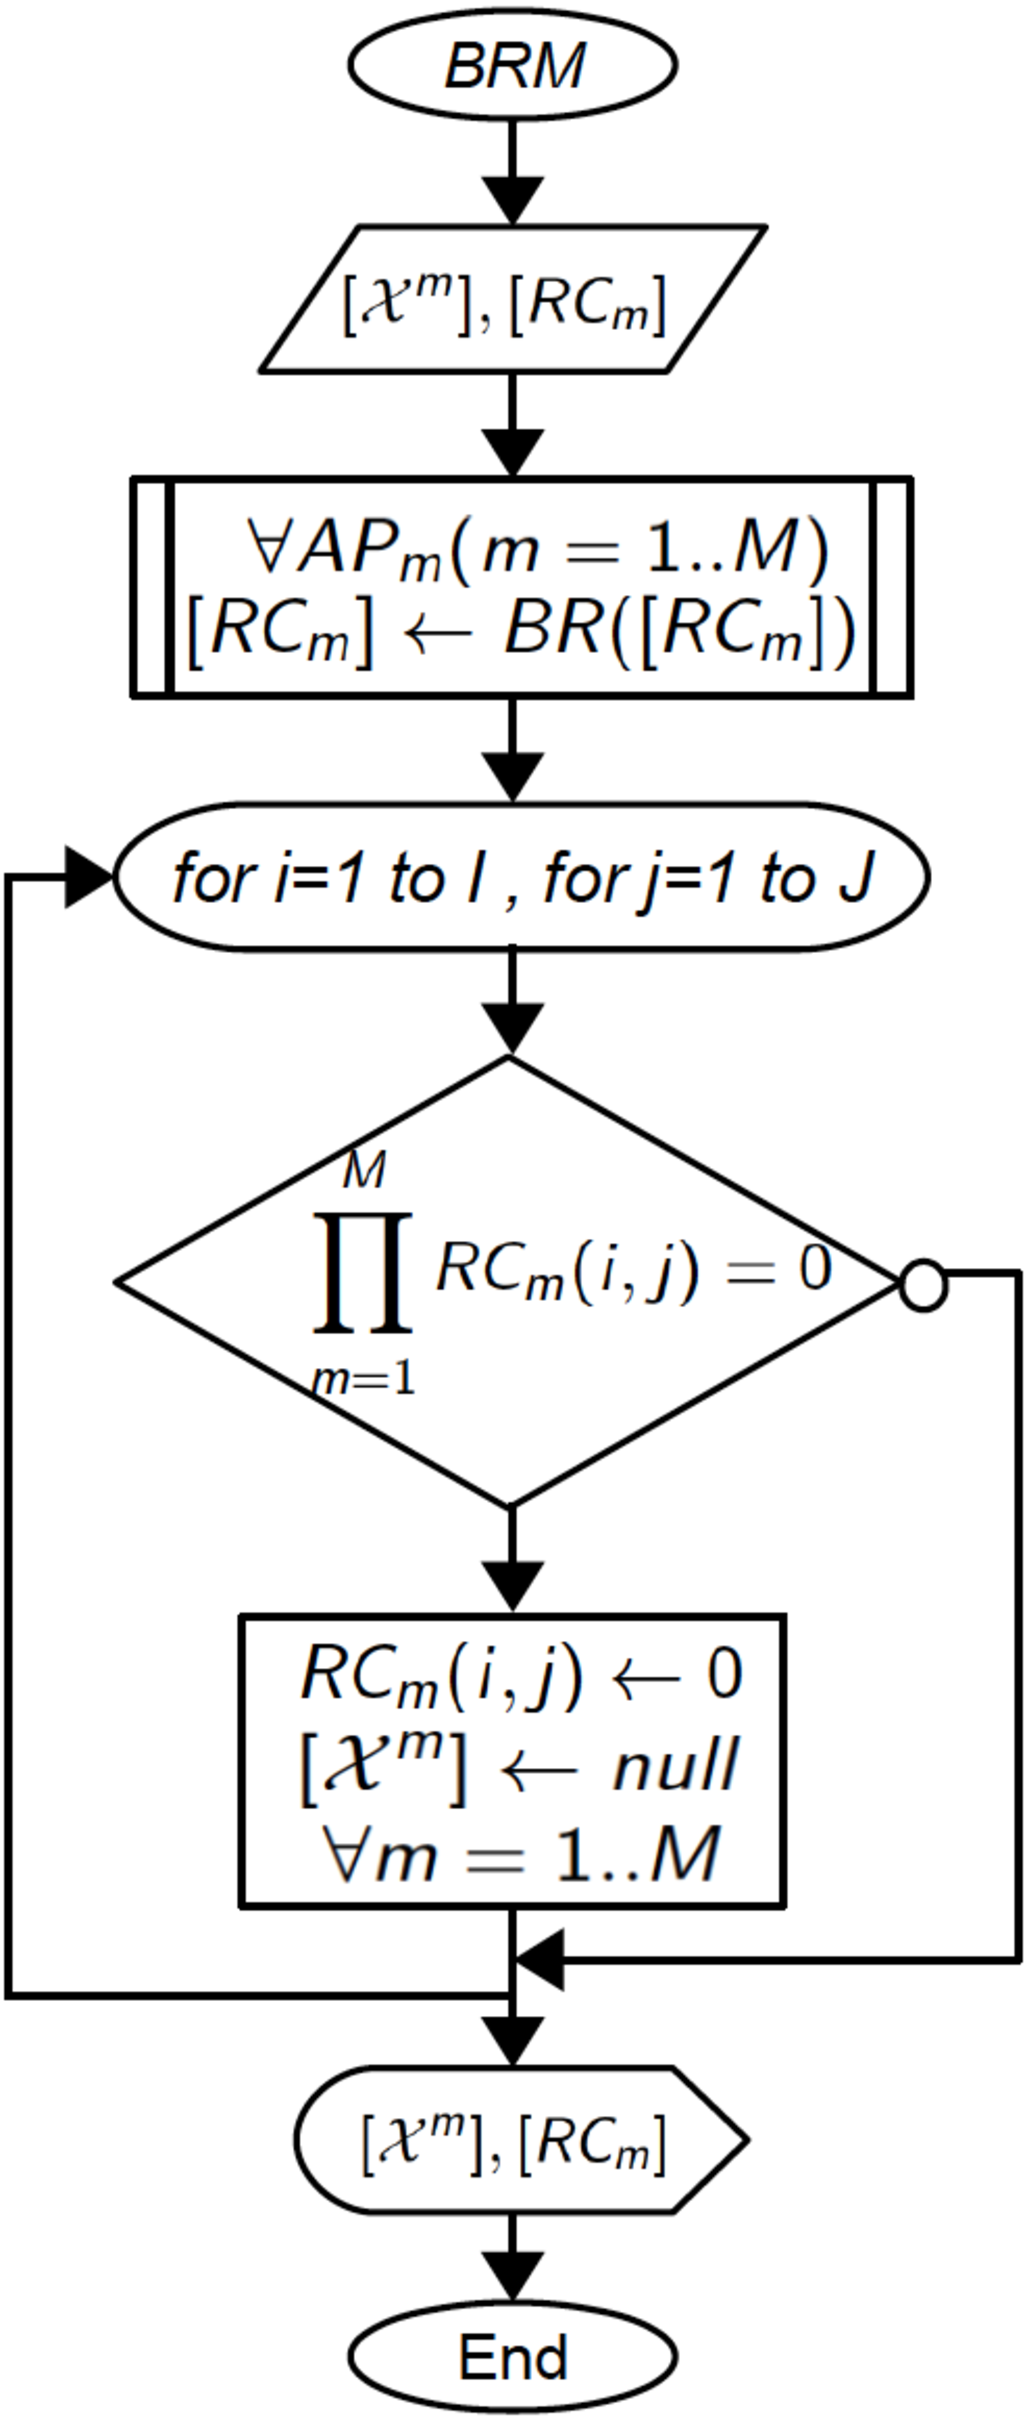
\includegraphics[width=0.322\textwidth]{figures/org-brm002}
					\hspace{0.8cm}
			}\hfill
			\caption{Illustration de l'utilisation de la méthode BRM}
			\label{org-brm}
		\end{center}
	\end{figure*}

La figure \ref{org-brm001} (de la page \pageref{org-brm001}) représente le premier organigramme et la figure \ref{org-brm002} (de la page \pageref{org-brm002}) le deuxième organigramme.

\subsection{Test des listings}

Présentation des principaux listings: les énumations et les listes.

\subsubsection{Énumérations: environement enum}

Test de l'environnement enum:
\begin{enumerate}
 \item test 1
 \item test 2
\end{enumerate}

\subsubsection{Listes: environement itemize}

Test de l'environnement itemize
\begin{itemize}
 \item test 1
 \item test 2
\end{itemize}

\subsection{Test des équations}

Mise en page des équations

\begin{equation}
   \beta = 8 \label{equation1}
\end{equation}

\begin{equation}
   \bm{\gamma} = \alpha \times 3
\end{equation} \label{equation2}

\subsection{Insertion d'une longue équation }

L'équation \ref{equation3} est un exemple d'équation, longue présentée sur plusieurs lignes.
    \begin{multline}
	C_m(SP_{\lambda}) = \Big(\underset{U_m \text{ fois }}{\underbrace{C_m(SP_1),..,C_m(SP_1)}}, ..,\\
	\underset{U_m \text{ fois }}{\underbrace{C_m(SP_{\lambda}),..,C_m(SP_{\lambda})}},...,\\
	\underset{U_m \text{ fois }}{\underbrace{C_m(SP_{\Lambda}),..,C_m(SP_{\Lambda})}}
	\Big) \label{equation3}
    \end{multline}


\section{Insertion d'algorithme }

\begin{algorithm}
    \KwData{\textbf{"Recursive Backtracking Algorithm"}}
	\vspace{0.2cm}
	\Pr{\textbf{Recursive-Backtracking}($\{\mathcal{X}\}$, $\{RC\}$)}{
		\KwIn{$\{\mathcal{X}\} ; \{RC\}$ : Resources Cost and Strategy
		}
		\KwOut{$\{\mathcal{X}\} ;\{RC\}$;
		}
		\textbf{Variable :}\\
			\ \ DominationExist = false;\\
		\For{$m = 1$ to $M$}{
			L = size of $[\mathcal{X}_m]$ of $AP_m$\\
			\For{l=1 to L-1}{
				\For{k=l+1 to L}{
					DSI$\big(\{\mathcal{X}^m_l\}$,$ [RC_l^m]$,$\{\mathcal{X}^m_k\}$,$ [RC_k^m],Domination\big)$\\
				}
			}
			\If{Domination}{
				DominationExist = true;\\
				Update($\{\mathcal{X}\}$, $\{RC\}$) of other players
			}
		}
		%Return the updated value of $\{\mathcal{X}\}$, $\{RC\}$\\
		\textbf{Return :}$\{\mathcal{X}\}$, $\{RC\}$ ;\\
		
		\If{DominationExist}{
			\textit{\textbf{Recursive-Backtracking}($\{\mathcal{X}\}$, $\{RC\}$);}
		}
	}
    \End
    \caption{"Recursive Backtracking Algorithm"\label{RecBack}} %
\end{algorithm}

L'algorithme a le numéro suivant \ref{RecBack} 

\lipsum[3]

\section{Seconde section}

Exemple de seconde section pour illustrer la mise en page de la table des matières